\chapter{Pomiary elektryczne tranzystorów}

W poniższym rozdziale omówiony zostanie układ pomiarowy, dzięki któremu możliwe było przeprowadzenie części eksperymetalnej
poniższej pracy. Następnie omówione zostaną charakterystyki elektryczne poszczególnych tranzystorów. Później opisany 
zostanie proces wygrzewania tranzystorów prądem o wysokiej gęstości. Omówione zostaną efekty takiego wygrzewania na 
zmiany w charakterystykach elektrycznych tranzystorów. Podjęta zostanie próba wyjaśnienia tego zjawiska. Na koniec 
pokazany zostanie wpływ wystawienia tak oczyszczonych tranzystorów na wpływ atmosfery, oraz jej wpływ na zmiany 
tychże charakterystyk.
	\section{Opis stanowiska pomiarowego}

	\begin{figure}[ht]
	\centering
	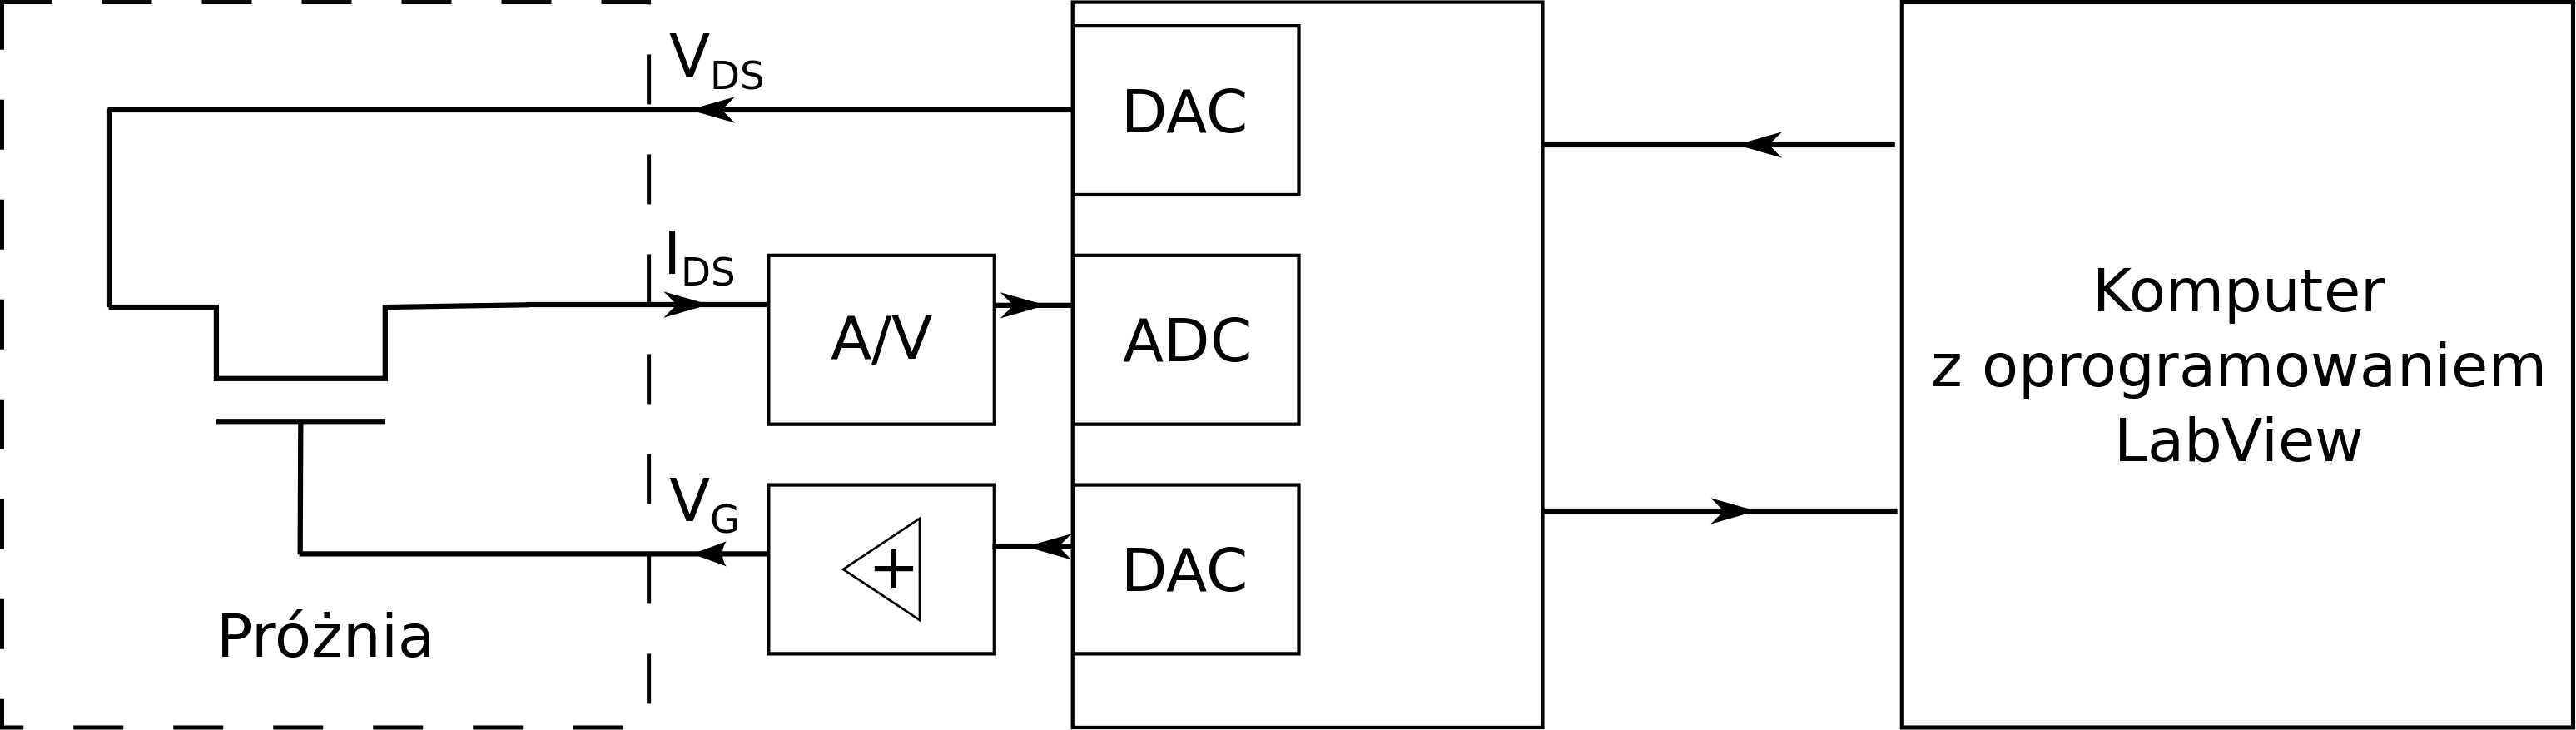
\includegraphics[width=1.0\textwidth]{./Rozdzial_4/obrazki/ukladblokowy.png}
	\caption{Schemat blokowy systemu pomiarowego}
	\label{fig:ukladblokowy}
	\end{figure}


	Na rysunku \ref{fig:ukladblokowy} został przedstawiony schemat blokowy systemu pomiarowego, użytego podczas zbierania danych 
	eksperymentalnych. Głównym elementem układu pomiarowego jest komputer osobisty z zainstalowanym
	oprogramowaniem LabView, które umożliwia sterowanie eksperymentem, akwizycję i archiwizację zebranych danych.
	
	Sterowanie odbywa się poprzez kartę rozszerzeń zapewniającą sterowanie napięciami drenu i bramkowego, 
	poprzez przetworniki cyfra-analog (\textit{ang. Digital-Analog-Converter}). Napięcia wychodzące z 
	karty mogą zmieniać się w zakresie $\pm$10 V. Dlatego do sterowania napięciem bramkowym użyto wzmacniacza, 
	o wzmocnieniu 20 razy. Zapewnia to możliwość uzyskania napięć bramkowych w zakresie $\pm$200 V. 
	Do sterowania napięciem drenu nie stosowano, żadnego dodatkowego wzmacniacza. Jedynie dla uzyskania 
	małych napięć dren-źródło stosowano dzielnik napięcia, który miał za zadanie niwelować wpływ przesunięć napięć
	spowodowanych niedoskonałością sprzętu pomiarowego. Ten problem zostanie opisany szerzej w następnym punkcie.

	Ostatnim ważnym aktywnym elementem pomiarowym jest wzmacniacz prąd ze zintegrowanym przetwornikiem 
	prąd-napięcie. Umożliwia on pomiar prądów rzędu pojedynczych pA. Sygnał wychodzący z tego wzmacniacza
	był następnie kierowany na przetwornik analog-cyfra (\textit{Analog-Digital-Converter}), znajdujący się
	w karcie pomiarowej komputera.

	Ostatnim elementem w układzie pomiarowym był kriostat zapewniający próżnię na odpowiednim poziomie. Okazało się,
	że część eksperymentalna związana z wygrzewaniem prądowym musi odbywać się w próżni. W przeciwnym wypadku
	tranzystory ulegały uszkodzeniom. Po zastosowaniu próżni nie zaobserwowano uszkodzenia tranzystorów. 
	By możliwe było umieszczenie próbki w kriostacie, niezbędne było wykonanie połączeń elektrycznych na drodze
	tak zwanego \textit{bondingu}. Następnie połączenia elektryczne zostały wyprowadzone na zewnątrz, przy pomocy 
	specjalnego uchwytu próbki. 



\begin{figure}[ht]
        \centering
        \begin{subfigure}[b]{0.7\textwidth}
              \centering
	\includegraphics[width=1\textwidth]{./Rozdzial_4/obrazki/uklad2.png}
	%\caption{Zdjęcie stanowiska pomiarowego wraz z odniesieniami do schematu blokowego}
	\label{fig:ukladzdjecie}
        \end{subfigure}%
        ~ %add desired spacing between images, e. g. ~, \quad, \qquad etc.
          %(or a blank line to force the subfigure onto a new line)
        \begin{subfigure}[b]{0.31\textwidth}
              \centering
	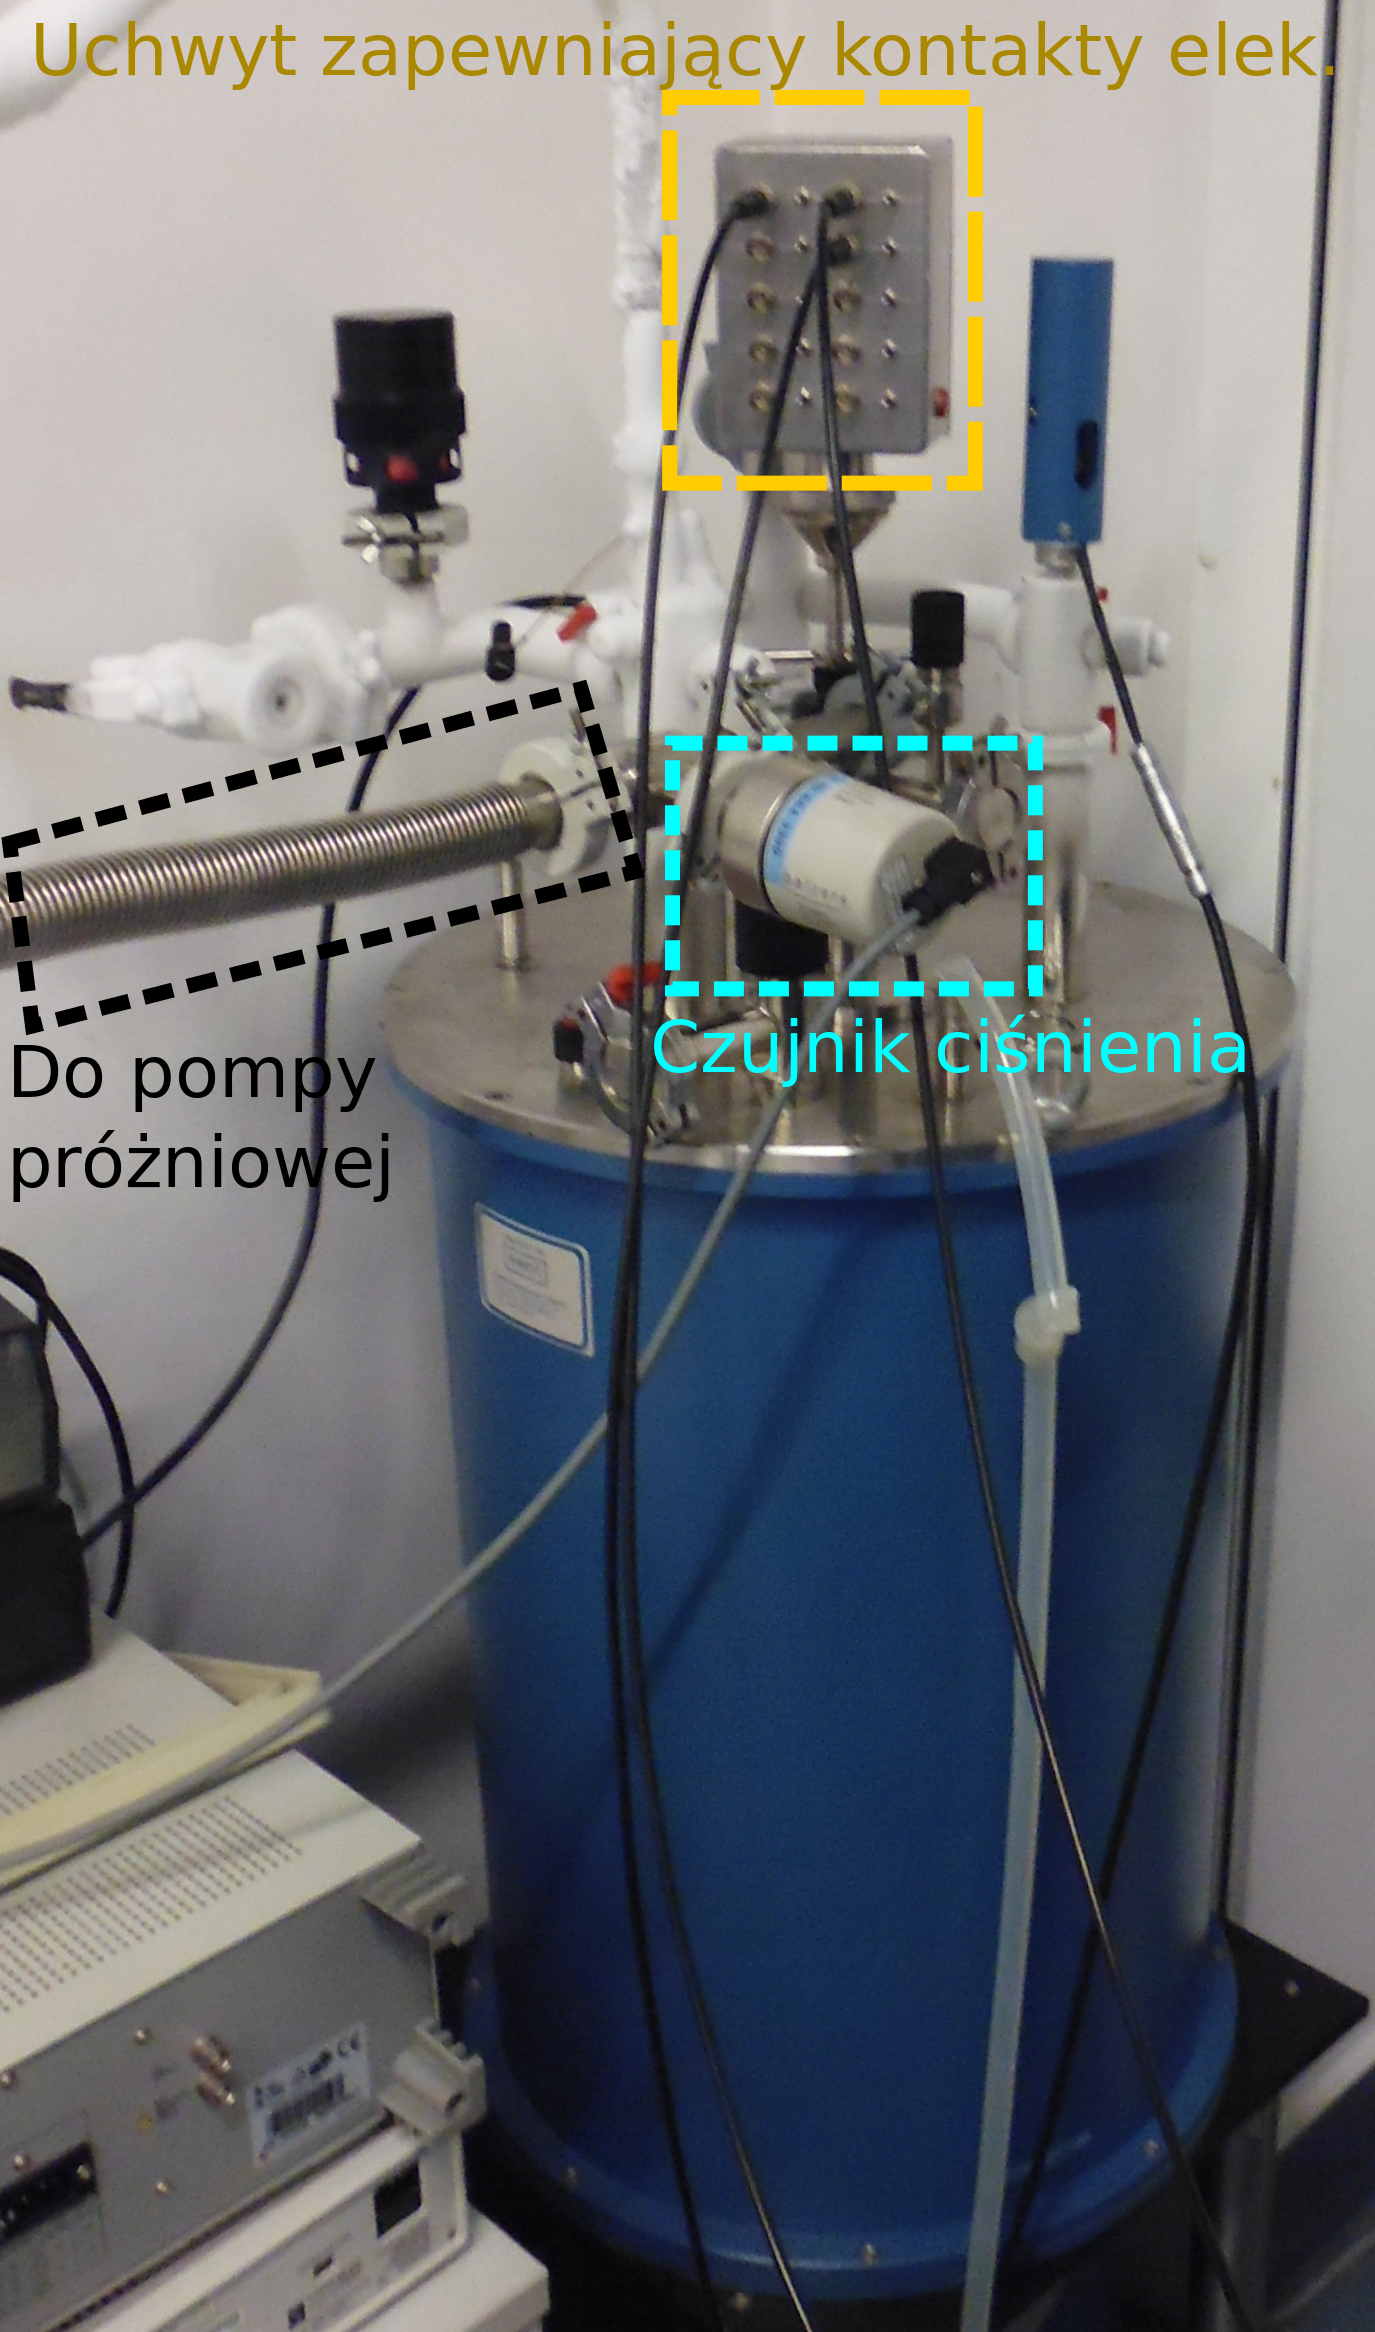
\includegraphics[width=1\textwidth]{./Rozdzial_4/obrazki/kriostat.png}
	%\caption{Zdjęcie stanowiska pomiarowego wraz z odniesieniami do schematu blokowego}
	\label{fig:ukladkriostat}
        \end{subfigure}
	\caption{Zdjęcie stanowiska pomiarowego wraz z odniesieniami do schematu blokowego}
\end{figure}

	\subsection{Rachunek niepewności}
	Każdy z elementów stanowiska pomiarowego wprowadza pewne zniekształcenia zaburzające pomiar. W przypadku użytych
	tutaj elementów wszystkie takiego zniekształcenia można opisać przy pomocy niepewności liniowych. To znaczy, 
	niepewność danej wielkości fizycznej opisywany jest przez funkcję w postaci
	 $\Delta x = \mathrm{a}\cdot x + \mathrm{b}$. Gdzie parametr a jest nazywany parametrem multiplikatywnym, 
	a parametr b jest nazywany addytywnym. 

	Na to wszystko nałożony jest również szum. W tym układzie szum jest różnorakiego pochodzenia: przydźwięk sieci
	energetycznej, szum samych urządzeń. By ustalić jakieś odniesienie co do stopnia zaszumienia, każdy pojedynczy 
	pomiar zakładał zebranie co najmniej tysiąca próbek, z przetwornika analogowo--cyfrowego. Następnie na podstawie
	tak zebranych danych liczona była średnia arytmetyczna i odchylenie standardowe. Średnia arytmetyczna, utożsamiona
	została z przybliżonym wynikiem pomiaru, natomiast średnia arytmetyczna stanowi przybliżenie niepewności losowej.
	
	\begin{table}[ht]
	\centering
	\begin{tabular}{l||c|c|r}
		Urządzenie & a & b & zakres \\
		\hline
		\hline
		DAC & $8\cdot 10^{-5}$ & 259 $\mu$V  & $\pm$10 V\\
			& $1,2\cdot 10^{-4}$ &	139 $\mu$V & $\pm$1 V\\
		\hline
		ADC & $6,7\cdot 10^{-5}$ & 290 $\mu$V & $\pm$10 V\\
		    & $6,7\cdot 10^{-5}$ &29 $\mu$V & $\pm$1 V\\
		\hline 
		A/V & $2\cdot 10^{-2}$ & 200 $\mu$V & cały zakres\\
	\end{tabular}
	\caption{ Zestawienie paramterów }
	\label{tab:blendy}
	\end{table}
	
	Podczas pomiarów charakterystyk przejściowych wykorzystywano trzy napięcia drenowe: 1 mV, 10 mV i 100 mV. 
	Natomiast zakresem napięć na bramce wynosił $\pm$60 V na bramce, czyli $\pm$3 V na przetworniku DAC.
	Charakterystyki wyjściowe wykorzystywały napięcia bramkowe również z takiego samego zakresu, natomiast 
	napięcia $\mathrm{V_{DS}}$ zawierały się w przedziale $\pm$100 mV.

	Porównując wartości przedstawione w tabelce \ref{tab:blendy}, można dojść do wniosku, że dla tych zakresów
	pomiarowych największe znaczenie mają stałe addytywne, zwane przesunięciami napięcia (\textit{offset voltage}).
	Przyczyny ich występowania są różne jednak w większości przypadków związane są z polaryzacją obwodów wejściowych
	wzmacniaczy operacyjnych znajdujących się na wejściu lub wyjściu urządzenia. 

	\section{Charakterystyki przejściowe i wyjściowe}
	\section{Proces wygrzewania prądowego tranzystorów grafenowych}
	\section{Ewolucja charakterystyk elektrycznych tranzystorów grafenowych wystawionych na działanie atmosfery}
